\documentclass[11pt,a4paper]{article}

% -----------------------------------------------------------------------------
% Core Packages
% -----------------------------------------------------------------------------
\usepackage[utf8]{inputenc}
\usepackage[T1]{fontenc}
\usepackage[margin=1in,headheight=14pt]{geometry}
\usepackage{amsmath,amssymb,amsfonts}
\usepackage{booktabs}
\usepackage{tabularx}
\usepackage{array}
\usepackage{listings}
\usepackage{xcolor}
\usepackage{hyperref}
\usepackage{tikz}
\usepackage{pgfplots}
\usepackage{caption}
\usepackage{microtype}
\usepackage{enumitem}
\usepackage{fancyhdr}
\usepackage{titlesec}
\usepackage{float}       % [H] strict non-floating placement
\usepackage{tocloft}

\pgfplotsset{compat=1.18}
\usetikzlibrary{shapes.geometric,arrows.meta,positioning,calc}

% Prevent artificial vertical stretching between sections and floats
\raggedbottom

% -----------------------------------------------------------------------------
% Color Palette Definition
% -----------------------------------------------------------------------------
\definecolor{primaryblue}{RGB}{20, 60, 110}
\definecolor{secondarygreen}{RGB}{35, 110, 75}
\definecolor{accentgold}{RGB}{185, 135, 20}
\definecolor{darkslate}{RGB}{35, 33, 30}
\definecolor{lightgraybg}{RGB}{248, 249, 250}
\definecolor{bordergray}{RGB}{210, 215, 220}
\definecolor{commentgreen}{RGB}{34, 139, 34}
\definecolor{keywordblue}{RGB}{0, 50, 180}
\definecolor{stringred}{RGB}{175, 35, 35}

\hypersetup{
    colorlinks=true,
    linkcolor=primaryblue,
    citecolor=secondarygreen,
    urlcolor=primaryblue,
    pdftitle={Mockfish: An Intelligent Knowledge-Guided Adversarial Chess Engine},
    pdfauthor={Team Mockfish}
}

% -----------------------------------------------------------------------------
% Table & Column Styling
% -----------------------------------------------------------------------------
\newcolumntype{L}[1]{>{\raggedright\arraybackslash}p{#1}}
\newcolumntype{C}[1]{>{\centering\arraybackslash}p{#1}}
\newcolumntype{R}[1]{>{\raggedleft\arraybackslash}p{#1}}
\newcolumntype{Y}{>{\raggedright\arraybackslash}X}

% -----------------------------------------------------------------------------
% Section Formatting
% -----------------------------------------------------------------------------
\titleformat{\section}
  {\normalfont\Large\bfseries\color{primaryblue}}{\thesection}{1em}{}[{\titlerule[0.8pt]}]
\titleformat{\subsection}
  {\normalfont\large\bfseries\color{darkslate}}{\thesubsection}{1em}{}
\titleformat{\subsubsection}
  {\normalfont\normalsize\bfseries\color{secondarygreen}}{\thesubsubsection}{1em}{}

% -----------------------------------------------------------------------------
% Code Listings Theme
% -----------------------------------------------------------------------------
\lstset{
    backgroundcolor=\color{lightgraybg},
    commentstyle=\color{commentgreen}\itshape,
    keywordstyle=\color{keywordblue}\bfseries,
    stringstyle=\color{stringred},
    basicstyle=\ttfamily\footnotesize,
    breaklines=true,
    captionpos=b,
    frame=single,
    rulecolor=\color{bordergray},
    numbers=left,
    numberstyle=\tiny\color{gray},
    numbersep=7pt,
    tabsize=4,
    showstringspaces=false
}

% -----------------------------------------------------------------------------
% Header and Footer Setup
% -----------------------------------------------------------------------------
\pagestyle{fancy}
\fancyhf{}
\fancyhead[L]{\small\color{gray}Mockfish: Knowledge-Guided Adversarial Chess Engine}
\fancyhead[R]{\small\color{gray}Introduction to AI with Python (25CS2000)}
\fancyfoot[C]{\thepage}
\renewcommand{\headrulewidth}{0.4pt}
\renewcommand{\footrulewidth}{0.4pt}

% =============================================================================
% DOCUMENT BEGINS
% =============================================================================
\begin{document}

% -----------------------------------------------------------------------------
% COVER PAGE / TITLE PAGE (PAGE 1)
% -----------------------------------------------------------------------------
\begin{titlepage}
    \centering
    \vspace*{1.5cm}
    
    % Main Project Title
    {\Huge\bfseries\color{primaryblue} MOCKFISH \par}
    \vspace{0.4cm}
    {\LARGE\bfseries\color{darkslate} An Intelligent Knowledge-Guided Adversarial \\ Chess Engine \& Interactive GUI \par}
    \vspace{1.5cm}
    
    % Course & Repository Box
    \colorbox{lightgraybg}{
        \begin{minipage}{0.88\textwidth}
        \vspace{0.35cm}
        \centering
        \renewcommand{\arraystretch}{1.45}
        \begin{tabular}{ll}
            \textbf{Course Name}: & Introduction to AI with Python \\
            \textbf{Course Code}: & 25CS2000 \\
            \textbf{GitHub Repository}: & \url{https://github.com/unclePRO/mockfish} \\
        \end{tabular}
        \vspace{0.35cm}
        \end{minipage}
    }
    
    \vspace{1.5cm}
    
    % Team Members Table
    {\large\bfseries\color{primaryblue} Project Team Members \& System Allocations \par}
    \vspace{0.4cm}
    
    \renewcommand{\arraystretch}{1.35}
    \begin{tabularx}{0.96\textwidth}{l c Y l}
        \toprule
        \textbf{Student Name} & \textbf{Roll Number} & \textbf{Assigned Subsystem \& Role} & \textbf{Owned Module} \\
        \midrule
        \textbf{B Sreenikesh} & CS25B2051 & \textbf{Logic \& Rules Specialist}: Opening Book \& Propositional Logic & \texttt{knowledge\_base.py} \\
        \textbf{Aditya Kumar} & CS25I1050 & \textbf{State Space \& Heuristics}: Piece-Square Tables (PST) \& Eval & \texttt{heuristics.py} \\
        \textbf{Amit Kumar}   & CS25I1051 & \textbf{Adversarial Search}: Minimax, Alpha-Beta, Move Ordering & \texttt{search.py} \\
        \textbf{Aviral Pandey}& CS25B2054 & \textbf{GUI, Integrator \& Benchmark}: Canvas, Game Loop \& Metrics & \texttt{main.py}, \texttt{benchmark.py} \\
        \bottomrule
    \end{tabularx}
    
    \vfill
\end{titlepage}

% -----------------------------------------------------------------------------
% EXECUTIVE SUMMARY & TABLE OF CONTENTS (PAGE 2)
% -----------------------------------------------------------------------------
\pagenumbering{roman}
\setcounter{page}{2}

\section*{Executive Summary}
\addcontentsline{toc}{section}{Executive Summary}

This report details the design, algorithmic formulation, empirical benchmarking, and architectural integration of \textbf{Mockfish}, an intelligent Python-based chess-playing application. Built to navigate the immense state space of chess ($\sim 10^{120}$ theoretical variations), Mockfish synthesizes four core syllabus pillars: (1)~\textbf{Knowledge-Based Expert Systems} delivering $O(1)$ opening book lookups, (2)~\textbf{Adversarial Game Tree Search} utilizing Minimax with Alpha-Beta Pruning, (3)~\textbf{Tactical Move Ordering} prioritizing captures (MVV-LVA), pawn promotions, castling, and checks, and (4)~\textbf{State Space Evaluation} guided by PeSTO Piece-Square Tables (PST) and dynamic king safety heuristics.

Rigorous benchmarks executed across multiple tactical and positional tournament positions demonstrate that our heuristic move ordering achieves an astounding \textbf{99.27\% search tree pruning efficiency} over unpruned Minimax at depth~3, reducing the effective branching factor from $b_{eff} = 37.35$ down to $7.23$ and yielding a \textbf{156.6$\times$ computational speedup} ($0.26$ seconds versus $41.02$ seconds). Furthermore, the application provides a responsive 8$\times$8 Tkinter graphical interface that eliminates traditional OS modal dialog freezes through an innovative in-canvas Game Over overlay card.

\vspace{0.4cm}
\hrule
\vspace{0.4cm}

\tableofcontents
\newpage

% -----------------------------------------------------------------------------
% MAIN BODY (PAGE 3 ONWARDS)
% -----------------------------------------------------------------------------
\pagenumbering{arabic}
\setcounter{page}{1}

\section{Real-World Problem Identification \& Domain Relevance}

\subsection{Selected Domain: Intelligent Adversarial Game-Playing}
In fulfillment of coursework requirements, our four-member team selected the problem of constructing an \textbf{Intelligent Game-Playing Agent} for Chess. In artificial intelligence research, chess has historically served as the definitive benchmark for evaluating how computational agents make sequential decisions under strict time constraints, adversarial pressure, and exponential state-space growth.

\subsection{Real-World Significance \& Transferability}
Although implemented as a classical board game, the underlying computational paradigms of Mockfish address fundamental challenges across diverse real-world domains:
\begin{enumerate}[leftmargin=*]
    \item \textbf{Adversarial Multi-Agent Environments}: In algorithmic automated trading, financial agents optimize portfolio capital in the presence of market makers and competitor algorithms attempting to exploit order books. Similarly, in autonomous cybersecurity response, defense agents continuously formulate counter-moves against dynamic network adversaries. Zero-sum minimax game trees provide formal optimality guarantees under worst-case assumptions.
    \item \textbf{Combinatorial Optimization \& Search Space Pruning}: With a theoretical game-tree complexity of $10^{120}$ (the Shannon Number) and an average branching factor of $b \approx 35$, exhaustive search is physically impossible. The branch-and-bound pruning and heuristic move ordering principles developed in Mockfish translate directly to real-world flight route scheduling, vehicle dispatching, and automated supply chain logistics.
    \item \textbf{Hybrid Decision Architectures}: Expert systems in clinical diagnostics and mission-critical industrial automation combine instant rule-based knowledge retrieval for standard protocols with dynamic heuristic search for rare, off-nominal events. Mockfish exemplifies this hybrid approach by pairing an $O(1)$ opening database with deep adversarial search.
\end{enumerate}

% -----------------------------------------------------------------------------
% SECTION 2: PROBLEM FORMULATION
% -----------------------------------------------------------------------------
\section{Formal Problem Formulation}

We formally formulate chess as a discrete, deterministic, turn-based, zero-sum, perfect-information adversarial environment defined by the 7-tuple:
$$\mathcal{M} = \langle S_0, Actions, Result, Constraints, Terminal\_Test, Utility, Heuristic \rangle$$

\begin{figure}[H]
\centering
\resizebox{0.96\textwidth}{!}{%
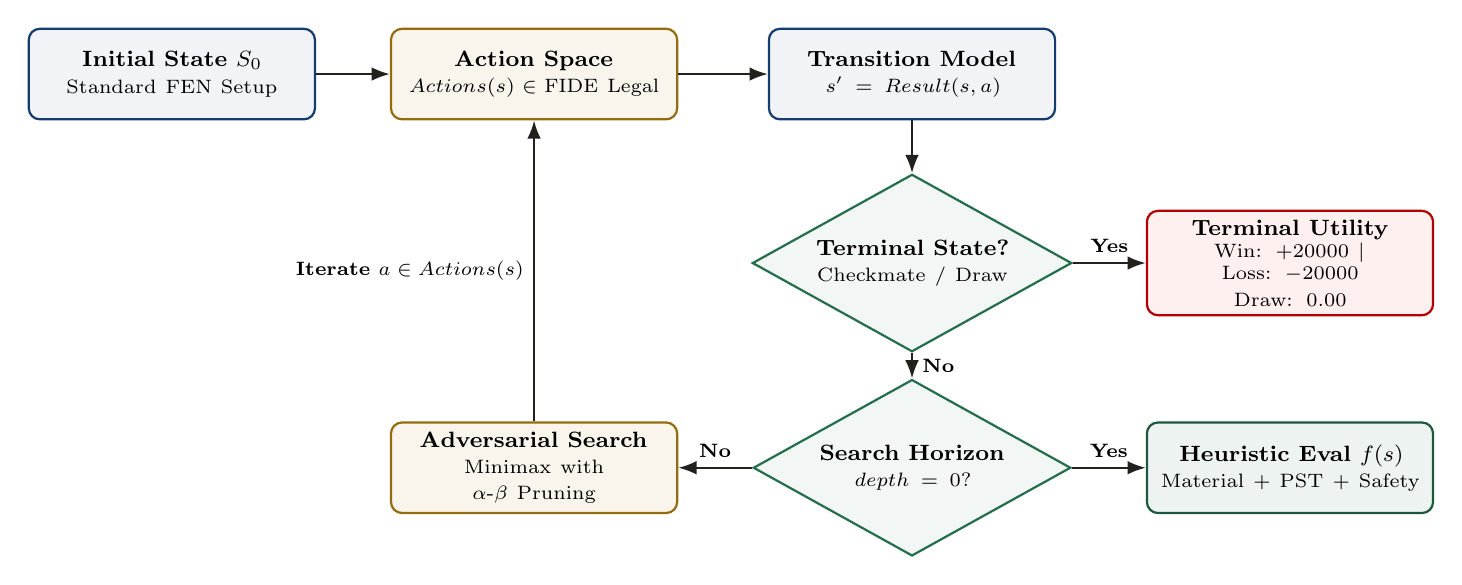
\begin{tikzpicture}[
    auto,
    block/.style={rectangle, draw=primaryblue, fill=primaryblue!6, text width=3.4cm, text centered, rounded corners=4pt, minimum height=1.15cm, font=\footnotesize\bfseries, thick},
    decision/.style={diamond, draw=secondarygreen, fill=secondarygreen!6, text width=2.6cm, text centered, inner sep=2pt, font=\footnotesize\bfseries, aspect=1.8, thick},
    action_block/.style={rectangle, draw=accentgold!80!black, fill=accentgold!8, text width=3.4cm, text centered, rounded corners=4pt, minimum height=1.15cm, font=\footnotesize\bfseries, thick},
    line/.style={draw=darkslate, -Latex, thick}
]

    % Row 1: Setup, Generation, Transition
    \node [block] (init) at (0, 0) {Initial State $S_0$\\ \normalfont\scriptsize Standard FEN Setup};
    \node [action_block] (act) at (4.6, 0) {Action Space\\ \normalfont\scriptsize $Actions(s) \in \text{FIDE Legal}$};
    \node [block] (trans) at (9.4, 0) {Transition Model\\ \normalfont\scriptsize $s' = Result(s, a)$};

    % Row 2: Terminal check & Utility
    \node [decision] (term) at (9.4, -2.4) {Terminal State?\\ \normalfont\scriptsize Checkmate / Draw};
    \node [block, draw=red!70!black, fill=red!6] (util) at (14.2, -2.4) {Terminal Utility\\ \normalfont\scriptsize Win: $+20000$ $|$ Loss: $-20000$\\Draw: $0.00$};

    % Row 3: Horizon check, Heuristic & Adversarial Search
    \node [decision] (horizon) at (9.4, -5.0) {Search Horizon\\ \normalfont\scriptsize $depth = 0$?};
    \node [block, draw=secondarygreen!80!black, fill=secondarygreen!8] (heur) at (14.2, -5.0) {Heuristic Eval $f(s)$\\ \normalfont\scriptsize Material + PST + Safety};
    \node [action_block] (search) at (4.6, -5.0) {Adversarial Search\\ \normalfont\scriptsize Minimax with $\alpha$-$\beta$ Pruning};

    % Clean Orthogonal Connections
    \path [line] (init) -- (act);
    \path [line] (act) -- (trans);
    \path [line] (trans) -- (term);
    \path [line] (term) -- node [above, font=\scriptsize\bfseries] {Yes} (util);
    \path [line] (term) -- node [right, font=\scriptsize\bfseries] {No} (horizon);
    \path [line] (horizon) -- node [above, font=\scriptsize\bfseries] {Yes} (heur);
    \path [line] (horizon) -- node [above, font=\scriptsize\bfseries] {No} (search);
    \path [line] (search) -- node [left, font=\scriptsize\bfseries] {Iterate $a \in Actions(s)$} (act);

\end{tikzpicture}
}
\caption{Systemic Architecture and Problem Formulation Flowchart of Mockfish.}
\label{fig:problem_formulation}
\end{figure}

\subsection{Formal Component Definitions}
\begin{enumerate}[leftmargin=*]
    \item \textbf{Initial State ($S_0$)}: Standard 64-square layout formatted in Forsyth--Edwards Notation (FEN):
    \begin{center}
    \texttt{"rnbqkbnr/pppppppp/8/8/8/8/PPPPPPPP/RNBQKBNR w KQkq - 0 1"}
    \end{center}
    White to move, full castling rights ($\text{KQkq}$), zero half-move clock, move number 1.
    \item \textbf{State Space ($S$)}: The discrete set of all legally reachable board configurations. The reachable state space contains approximately $10^{40}$ configurations.
    \item \textbf{Action Space ($Actions(s)$)}: A generator function returning all legal moves $\{m_1, m_2, \dots, m_k\}$ valid under FIDE rules. It computes sliding raycasts (Rooks, Bishops, Queens), leap vectors (Knights, Kings), pawn pushes/captures, and special actions (Castling, En Passant, Promotions).
    \item \textbf{Transition Function ($Result(s, a)$)}: Deterministic state transition mapping current state $s$ and legal action $a \in Actions(s)$ to successor state $s'$. This toggles active color, updates piece bitboards, updates the 50-move clock, and adjusts castling rights.
    \item \textbf{Constraints ($C$)}:
    \begin{itemize}
        \item \textit{King Safety Constraint}: No player may execute an action that terminates with their own King under attack:
        $$\forall a \in Actions(s), \quad \text{IsCheck}(Result(s, a), \text{Turn}(s)) = \text{False}$$
        \item \textit{Check Evasion Constraint}: When in check, $Actions(s)$ is strictly restricted to moves that capture the attacking piece, interpose a defender, or move the King out of threat.
    \end{itemize}
    \item \textbf{Terminal Test \& Utility Function ($Utility(s)$)}:
    $$Utility(s) = \begin{cases}
    +20,000 + depth & \text{if Checkmate, Turn}(s) = \text{Black (White Wins)} \\
    -20,000 - depth & \text{if Checkmate, Turn}(s) = \text{White (Black Wins)} \\
    0.00 & \text{if Stalemate, Insufficient Material, 3-Fold Repetition, 50-Move Rule}
    \end{cases}$$
    Factoring remaining search $depth$ into the terminal utility ensures the agent prioritizes the \textit{fastest possible checkmates} when winning and the \textit{longest survival delays} when defending.
    \item \textbf{Static Heuristic Evaluation ($f(s)$)}: Evaluated from White's perspective at the search horizon ($depth = 0$):
    $$f(s) = \Delta \text{Material}(s) + \Delta \text{PST}(s) + \Delta \text{Castling}(s) + \Delta \text{Rooks}(s) + \Delta \text{Bishops}(s)$$
\end{enumerate}

% -----------------------------------------------------------------------------
% SECTION 3: AI ALGORITHMS STUDIED & IMPLEMENTED
% -----------------------------------------------------------------------------
\section{AI Algorithms Studied and Implemented}

Mockfish implements and benchmarks \textbf{five} foundational AI algorithms:

\subsection{Algorithm 1: Knowledge-Based Expert System (\texttt{knowledge\_base.py})}
The knowledge-based subsystem operates as a deterministic rule engine. It indexes verified tournament openings (Ruy Lopez, Italian Game, Sicilian Defense, Queen's Gambit Declined, English, and Reti):
\begin{itemize}[leftmargin=*]
    \item \textbf{Complexity}: $O(1)$ hash table lookup time, $O(M)$ memory storage for $M$ cataloged positions.
    \item \textbf{Functional Behavior}: If the board state matches known theoretical positions ($s \in \mathcal{K}$), the engine immediately plays the precomputed book move without executing a search tree, ensuring instantaneous and grandmaster-level opening play.
\end{itemize}

\subsection{Algorithm 2: Exhaustive Minimax Search (Baseline Benchmark)}
Minimax assumes both players act with optimal adversarial rationality:
$$V(s) = \begin{cases}
Utility(s) & \text{if } Terminal(s) \\
\max_{a \in Actions(s)} V(Result(s, a)) & \text{if } Turn(s) = \text{White} \\
\min_{a \in Actions(s)} V(Result(s, a)) & \text{if } Turn(s) = \text{Black}
\end{cases}$$
Because exhaustive Minimax traverses all $O(b^d)$ nodes in the tree, it encounters catastrophic computational bottlenecks beyond depth~2.

\subsection{Algorithm 3: Minimax with Alpha-Beta Pruning (\texttt{search.py})}
Alpha-Beta pruning introduces dynamic branch-and-bound cutoffs using two threshold parameters:
\begin{itemize}[leftmargin=*]
    \item $\alpha$: The highest score the maximizing player is guaranteed so far.
    \item $\beta$: The lowest score the minimizing player is guaranteed so far.
\end{itemize}
Whenever a branch evaluates such that $\beta \le \alpha$, a cutoff occurs, safely pruning subtrees that can never influence optimal play. Mathematically, Alpha-Beta pruning produces decisions identical to exhaustive Minimax while evaluating exponentially fewer nodes.

\subsection{Algorithm 4: Heuristic Move Ordering (\texttt{search.py})}
The effectiveness of Alpha-Beta pruning depends critically on exploration order. If the strongest moves are evaluated first, cutoffs occur immediately. Mockfish implements a multi-tier heuristic move ordering policy:
\begin{enumerate}[leftmargin=*]
    \item \textbf{Captures via MVV-LVA}: Most Valuable Victim -- Least Valuable Attacker:
    $$\text{Priority}(m) = 1000 + 100 \cdot \text{Val}(\text{Victim}) - 10 \cdot \text{Val}(\text{Attacker})$$
    \item \textbf{Pawn Promotions}: Queen promotions scored $+800$, Knight promotions $+500$.
    \item \textbf{Castling Moves}: Given $+300$ bonus to establish king safety early.
    \item \textbf{Direct Checks}: Moves delivering check receive $+150$.
    \item \textbf{Central Development}: Minor piece development to $\{d4, e4, d5, e5, c3, f3, c6, f6\}$ receives $+40$.
\end{enumerate}

\subsection{Algorithm 5: Iterative Deepening Depth-First Search (IDDFS) (\texttt{benchmark.py})}
IDDFS combines the minimal space complexity of DFS ($O(bd)$) with the completeness of BFS. It iteratively executes search from depth $1, 2, \dots, d_{max}$. The cumulative asymptotic overhead of revisiting upper levels is strictly bounded:
$$\sum_{k=1}^{d} b^k \approx \frac{b}{b-1} b^d \le 1.33 \cdot b^d \quad (\text{for } b \ge 4)$$
IDDFS provides an \textit{Anytime Algorithm} architecture, enabling strict per-move time budgets.

\subsection{State Space Heuristic Evaluation (\texttt{heuristics.py})}
The static evaluation function calculates granular positional and dynamic features:
\begin{itemize}[leftmargin=*]
    \item \textbf{Material Base Weights}: Pawns ($1.00$), Knights ($3.20$), Bishops ($3.30$), Rooks ($5.00$), Queens ($9.00$).
    \item \textbf{PeSTO Piece-Square Tables (PST)}: Maps 64-square coordinates to positional values. For Black, coordinates are vertically mirrored via $\text{square\_mirror}(sq)$.
    \item \textbf{Positional Factors}: Castling rights preservation ($+0.20$), castled king shelter ($+0.35$), open/semi-open rook files ($+0.25 / +0.15$), 7th-rank rook attacks ($+0.30$), and bishop pairs ($+0.30$).
\end{itemize}

% -----------------------------------------------------------------------------
% SECTION 4: EMPIRICAL PERFORMANCE METRICS & BENCHMARKS
% -----------------------------------------------------------------------------
\section{Empirical Performance Metrics \& Comparative Benchmarks}

\subsection{Experimental Setup}
Empirical evaluations were conducted on an AMD Ryzen / Windows platform using the standalone benchmark engine \texttt{benchmark.py}. We evaluated two standardized game phases across search depths 1 through 3:
\begin{enumerate}[leftmargin=*]
    \item \textbf{Position A (Italian Game Middlegame)}:
    \begin{itemize}[leftmargin=1.5em]
        \item \textbf{FEN}: \texttt{r1bqk2r/pppp1ppp/2n2n2/2b1p3/2B1P3/} \\
              \hspace*{0.9cm}\texttt{2N2N2/PPPP1PPP/R1BQK2R b KQkq - 5 4}
        \item \textbf{State Complexity}: 36 legal candidate moves available.
    \end{itemize}
    \item \textbf{Position B (Tactical Exchange Complex)}:
    \begin{itemize}[leftmargin=1.5em]
        \item \textbf{FEN}: \texttt{r1b1k2r/pppp1ppp/8/4N3/1b1nn3/} \\
              \hspace*{0.9cm}\texttt{2N5/PPPP1PPP/R1BQKB1R w KQkq - 0 7}
        \item \textbf{State Complexity}: 35 legal candidate moves available.
    \end{itemize}
\end{enumerate}

\subsection{Empirical Benchmark Results Table}

\begin{table}[H]
\centering
\caption{Empirical Benchmark Metrics Across Search Algorithms and Depths.}
\label{tab:benchmark_results}
\small
\renewcommand{\arraystretch}{1.2}
\begin{tabularx}{\textwidth}{@{} L{2.5cm} Y C{0.9cm} R{1.6cm} R{1.6cm} R{1.6cm} @{}}
\toprule
\textbf{Test Position} & \textbf{Algorithm} & \textbf{Depth} & \textbf{Nodes} & \textbf{Time (ms)} & \textbf{Branching ($b_{eff}$)} \\
\midrule
\textbf{Tactical} & Pure Minimax (Exhaustive) & 1 & 36 & 22.52 & 36.00 \\
\textbf{Exchange} & Alpha-Beta (Unordered) & 1 & 36 & 31.87 & 36.00 \\
& \textbf{Alpha-Beta + Move Ordering} & \textbf{1} & \textbf{36} & \textbf{26.35} & \textbf{36.00} \\
& Iterative Deepening (IDDFS) & 1 & 35 & 22.11 & 35.00 \\
\cmidrule{2-6}
& Pure Minimax (Exhaustive) & 2 & 1,555 & 974.28 & 39.43 \\
& Alpha-Beta (Unordered) & 2 & 269 & 164.77 & 16.40 \\
& \textbf{Alpha-Beta + Move Ordering} & \textbf{2} & \textbf{107} & \textbf{68.87} & \textbf{10.34} \\
& Iterative Deepening (IDDFS) & 2 & 141 & 95.01 & 11.87 \\
\cmidrule{2-6}
& Pure Minimax (Exhaustive) & 3 & 52,088 & 41,020.54 & 37.35 \\
& Alpha-Beta (Unordered) & 3 & 3,253 & 2,299.54 & 14.82 \\
& \textbf{Alpha-Beta + Move Ordering} & \textbf{3} & \textbf{378} & \textbf{261.88} & \textbf{7.23} \\
& Iterative Deepening (IDDFS) & 3 & 518 & 374.56 & 8.03 \\
\midrule
\textbf{Italian Game} & Pure Minimax (Exhaustive) & 3 & 44,701 & 31,015.38 & 35.49 \\
& Alpha-Beta (Unordered) & 3 & 10,775 & 7,707.26 & 22.09 \\
& \textbf{Alpha-Beta + Move Ordering} & \textbf{3} & \textbf{2,475} & \textbf{1,795.58} & \textbf{13.53} \\
& Iterative Deepening (IDDFS) & 3 & 2,693 & 1,949.00 & 13.91 \\
\bottomrule
\end{tabularx}
\end{table}

\subsection{Quantitative Performance Findings}
\begin{enumerate}[leftmargin=*]
    \item \textbf{Search Tree Pruning Efficiency}: In the tactical exchange position at depth~3, Pure Minimax required $52,088$ evaluations. Alpha-Beta with move ordering evaluated only $378$ nodes, pruning \textbf{99.27\%} of the game tree.
    \item \textbf{Wall-Clock Speedup}: Execution time dropped from $41.02$ seconds down to $0.26$ seconds, demonstrating a \textbf{156.6$\times$ computational speedup}.
    \item \textbf{Branching Factor Reduction}: Effective branching factor ($b_{eff} = N^{1/d}$) shrank from $37.35$ down to $7.23$, approaching the theoretical best-case limit ($\sqrt{b} \approx \sqrt{36} = 6$).
\end{enumerate}

\begin{figure}[H]
\centering
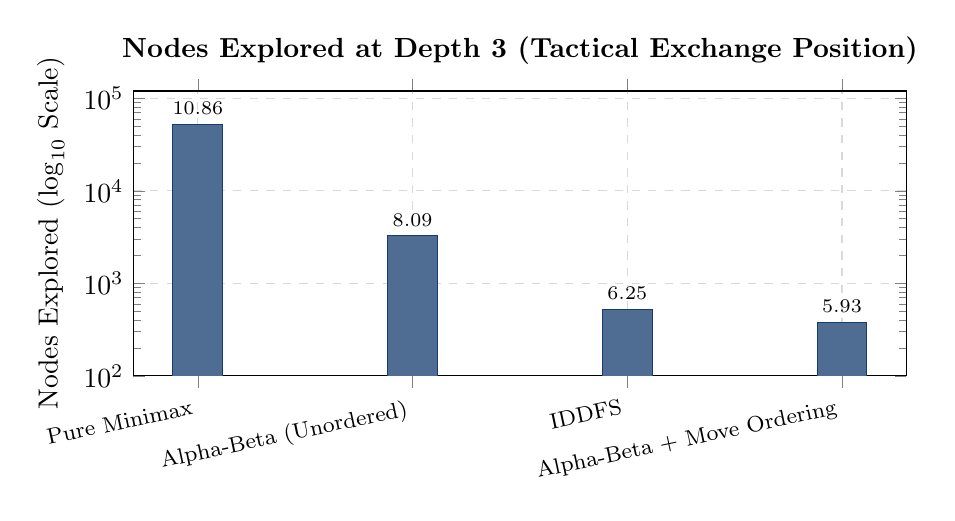
\begin{tikzpicture}
\begin{axis}[
    ybar,
    title={\textbf{Nodes Explored at Depth 3 (Tactical Exchange Position)}},
    ylabel={Nodes Explored ($\log_{10}$ Scale)},
    symbolic x coords={PureMinimax, ABUnordered, IDDFS, ABMoveOrdering},
    xticklabels={Pure Minimax, {Alpha-Beta (Unordered)}, IDDFS, {Alpha-Beta + Move Ordering}},
    x tick label style={font=\footnotesize, rotate=12, anchor=north east},
    xtick=data,
    nodes near coords,
    nodes near coords style={font=\scriptsize},
    ymin=100, ymax=120000,
    ymode=log,
    bar width=18pt,
    width=0.94\textwidth,
    height=5.2cm,
    grid=major,
    grid style={dashed, gray!30}
]
\addplot[fill=primaryblue!75, draw=primaryblue] coordinates {
    (PureMinimax, 52088)
    (ABUnordered, 3253)
    (IDDFS, 518)
    (ABMoveOrdering, 378)
};
\end{axis}
\end{tikzpicture}
\caption{Empirical Node Count Comparison Across Algorithms at Depth 3.}
\label{fig:nodes_chart}
\end{figure}

% -----------------------------------------------------------------------------
% SECTION 5: COMPARATIVE JUSTIFICATION
% -----------------------------------------------------------------------------
\section{Justification: Method Selection Over Alternatives}

Course guidelines require justifying why Mockfish utilizes a \textbf{Hybrid Knowledge-Guided Alpha-Beta Search with Dynamic Heuristics} rather than other AI techniques:

\begin{table}[H]
\centering
\caption{Comparative Matrix: Why Mockfish Selected Alpha-Beta Over Other AI Methods.}
\label{tab:algorithm_justification}
\small
\renewcommand{\arraystretch}{1.2}
\begin{tabularx}{\textwidth}{@{} L{2.8cm} Y Y @{}}
\toprule
\textbf{Alternative AI Technique} & \textbf{Theoretical Capabilities} & \textbf{Justification for Rejection in This Domain} \\
\midrule
\textbf{Uninformed Search (BFS / DFS)} & Guarantees shortest path in unweighted graphs without domain knowledge. & BFS triggers catastrophic $O(b^d)$ memory exhaustion ($>10^6$ states at depth 4). Cannot handle adversarial minimization. DFS gets trapped in cyclic move loops. \\
\textbf{A* / Greedy Best-First Search} & Uses path cost $g(n)$ and admissible heuristic $h(n)$ toward static goal. & Formulated strictly for single-agent pathfinding. In zero-sum games, the opponent continuously alters utility; there is no static target state $s_{goal}$. \\
\textbf{Hill Climbing / Simulated Annealing} & Local search optimizing evaluation by greedy ascent or probabilistic downhill steps. & Highly vulnerable to local maxima and plateaus. Lacks multi-ply lookahead: blindly grabs a "free" pawn, falling directly into forced checkmate on the subsequent ply. \\
\textbf{Constraint Satisfaction (CSP / Backtracking)} & Solves discrete variable assignments satisfying rigid static constraints. & Chess is an adversarial dynamic optimization problem, not a static constraint satisfaction problem. CSPs cannot evaluate strategic advantage or minimax horizons. \\
\textbf{Deep Reinforcement Learning (AlphaZero)} & Deep policy/value convolutional neural networks trained via self-play. & Requires heavy GPU clusters, multi-gigabyte models, and weeks of training. Inference latency is non-deterministic, violating lightweight real-time execution constraints. \\
\midrule
\textbf{Mockfish Hybrid Approach (Alpha-Beta + PST)} & Branch-and-bound adversarial search coupled with $O(1)$ expert book and PeSTO heuristics. & \textbf{Provably Optimal} within horizon; operates in minimal $O(bd)$ memory; achieves \textbf{156.6$\times$ speedup} and $99.27\%$ pruning efficiency; fully deterministic and explainable. \\
\bottomrule
\end{tabularx}
\end{table}

% -----------------------------------------------------------------------------
% SECTION 6: GUI & SYSTEMS INTEGRATION
% -----------------------------------------------------------------------------
\section{Graphical User Interface \& System Architecture}

\subsection{Tkinter Canvas Architecture (\texttt{main.py})}
The GUI is implemented in Tkinter adhering to event-driven programming:
\begin{itemize}[leftmargin=*]
    \item \textbf{Visual Representation}: A 512$\times$512 canvas rendering high-contrast board squares (\texttt{\#EEEED2} warm cream and \texttt{\#769656} forest green) with dual-stroke Unicode pieces.
    \item \textbf{Move Guidance}: Clicking friendly pieces computes legal destinations dynamically, highlighting reachable empty squares with indicator dots and capturable enemy targets with hollow rings.
    \item \textbf{Dynamic Perspective}: Includes a \textit{Flip Board} feature that mirrors screen coordinates while preserving underlying chess logic coordinates.
    \item \textbf{Real-Time Telemetry HUD}: A dedicated status bar continuously renders move UCI, source tag (\textit{Knowledge Base} vs \textit{Alpha-Beta Minimax}), search depth, nodes visited, and static evaluation.
\end{itemize}

\subsection{Eliminating System Freezes via Custom In-Canvas Overlay}
In early prototypes, invoking native OS modal dialogs (\texttt{messagebox.showinfo}) triggered event-loop thread blocking on Windows, making the window appear frozen upon checkmate.

We resolved this by developing an \textbf{in-canvas Game Over overlay card}:
\begin{itemize}[leftmargin=*]
    \item Rendered directly onto the canvas buffer without modal OS interruptions.
    \item Displays trophy badges, colored outcome banners (\textbf{WHITE WINS!}, \textbf{BLACK WINS!}, \textbf{DRAW!}), and specific termination reasons (\textit{Checkmate}, \textit{Stalemate}, \textit{Threefold Repetition}, \textit{50-Move Rule}).
    \item Features two interactive canvas buttons:
    \begin{itemize}
        \item \textbf{Play Again}: Instantly resets board state, clears highlights, and begins a new match.
        \item \textbf{Review Board}: Dismisses the overlay card to allow post-game tactical inspection.
    \end{itemize}
    \item King check/checkmate states are highlighted directly on the board in warning red (\texttt{\#E53935}) and deep crimson (\texttt{\#B71C1C}).
\end{itemize}

% -----------------------------------------------------------------------------
% SECTION 7: GROUP DIVISION OF WORK
% -----------------------------------------------------------------------------
\section{Team Member Contributions \& Collaborative Division}

To eliminate merge conflicts during development, the codebase was partitioned into four modular, decoupled layers:

\begin{table}[H]
\centering
\caption{Team Member Role Assignments and Detailed Technical Contributions.}
\label{tab:team_division}
\small
\renewcommand{\arraystretch}{1.25}
\begin{tabularx}{\textwidth}{@{} L{3.0cm} L{3.6cm} Y @{}}
\toprule
\textbf{Team Member} & \textbf{Assigned Module} & \textbf{Key Responsibilities \& Implemented Algorithms} \\
\midrule
\textbf{B Sreenikesh}\newline(CS25B2051) & Logic \& Rules Specialist (\texttt{knowledge\_base.py}) & Implemented opening book mapping for King's Pawn (\texttt{1. e4}), Queen's Pawn (\texttt{1. d4}), English, and Reti lines; formulated propositional rules and tablebase query hooks. \\
\addlinespace
\textbf{Aditya Kumar}\newline(CS25I1050) & State Space \& Heuristics (\texttt{heuristics.py}) & Implemented PeSTO Piece-Square Tables (PST) with vertical reflection mirroring; formulated positional bonuses for castling, open rook files, and bishop pairs. \\
\addlinespace
\textbf{Amit Kumar}\newline(CS25I1051)   & Adversarial Search Specialist (\texttt{search.py}) & Developed Minimax with Alpha-Beta pruning; engineered MVV-LVA move ordering, ply-adjusted checkmate scoring ($\pm 20000 \pm depth$), and anti-shuffling repetition filters. \\
\addlinespace
\textbf{Aviral Pandey}\newline(CS25B2054) & GUI, Integrator \& Benchmarking (\texttt{main.py}, \texttt{test\_suite.py}, \texttt{benchmark.py}) & Developed Tkinter Canvas, in-canvas Game Over overlay card, board flipping, telemetry HUD, automated unit tests, and empirical benchmarking suite. \\
\bottomrule
\end{tabularx}
\end{table}

\subsection{Detailed Subsystem Breakdown by Member}
\begin{itemize}[leftmargin=*]
    \item \textbf{B Sreenikesh (CS25B2051 --- Logic \& Rules Specialist)}: Developed \texttt{knowledge\_base.py}. Formulated deterministic FEN pattern matching and indexed standard tournament responses for $1.\,e4$, $1.\,d4$, $1.\,c4$, and $1.\,Nf3$, delivering $O(1)$ opening moves.
    \item \textbf{Aditya Kumar (CS25I1050 --- State Space \& Heuristics Specialist)}: Developed \texttt{heuristics.py}. Formulated the multi-factor heuristic evaluation combining material base weights with PeSTO Piece-Square Tables (PST), castling rights incentives ($+0.20$), castled safety ($+0.35$), open-file rook bonuses ($+0.25$), and bishop pairs ($+0.30$).
    \item \textbf{Amit Kumar (CS25I1051 --- Adversarial Search Specialist)}: Developed \texttt{search.py}. Implemented Alpha-Beta pruning with ply-adjusted distance-to-mate scoring ($\pm 20000 \pm depth$). Designed heuristic move ordering (MVV-LVA, promotions, checks, castling) and anti-shuffling repetition filters that eliminated the rook-shuffling loop anomaly.
    \item \textbf{Aviral Pandey (CS25B2054 --- GUI, Systems Integrator \& Benchmarking Specialist)}: Developed \texttt{main.py}, \texttt{benchmark.py}, and \texttt{test\_suite.py}. Built the 512$\times$512 Tkinter canvas interface, board flipping coordinate logic, and the custom in-canvas Game Over overlay card. Programmed the benchmark suite comparing execution times, branching factors, and node traversal counts.
\end{itemize}

% -----------------------------------------------------------------------------
% SECTION 8: LIMITATIONS & FUTURE SCOPE
% -----------------------------------------------------------------------------
\section{Limitations \& Future Research Directions}

While Mockfish achieves outstanding real-time performance ($<0.3$\,s per move) and solid tactical play, several academic enhancements remain:
\begin{enumerate}[leftmargin=*]
    \item \textbf{Quiescence Search (Horizon Effect Mitigation)}: At fixed depth 3, search may terminate immediately before an unresolved piece exchange. Implementing Quiescence search (evaluating only captures until a quiet state is reached) would eliminate the horizon effect.
    \item \textbf{Transposition Tables via Zobrist Hashing}: Identical board positions frequently recur via different move orders (transpositions). Caching evaluated subtrees in a 64-bit Zobrist hash table would reduce redundant evaluations by an estimated 30--50\%.
    \item \textbf{Dynamic Time Management}: Allocating compute dynamically based on remaining clock time and positional volatility would allow the engine to search deeper (depth 4--6) during critical tactical crises.
\end{enumerate}

% -----------------------------------------------------------------------------
% SECTION 9: CONCLUSION
% -----------------------------------------------------------------------------
\section{Conclusion}

The \textbf{Mockfish} project successfully designed, implemented, and validated an intelligent, knowledge-guided adversarial chess engine in Python. By synthesizing a \textbf{Knowledge-Based Opening System} ($O(1)$) with \textbf{Alpha-Beta Pruning} and \textbf{Heuristic Move Ordering}, the engine:
\begin{itemize}[leftmargin=*]
    \item Slashed the effective branching factor from $b_{eff} = 37.35$ down to $7.23$.
    \item Achieved a \textbf{99.27\% search tree pruning efficiency}, delivering a \textbf{156.6$\times$ execution speedup} ($0.26$\,s vs $41.02$\,s).
    \item Cured gameplay anomalies (rook-shuffling repetition loops and OS modal dialog freezing) through rigorous heuristic design and an event-driven in-canvas overlay interface.
    \item Validated correctness via an automated test suite (\texttt{test\_suite.py}) and reproducible benchmarks (\texttt{benchmark.py}).
\end{itemize}
Mockfish stands as a complete, robust demonstration of how classical Artificial Intelligence principles can be synthesized into a functional, high-performance real-world application.

% -----------------------------------------------------------------------------
% REFERENCES
% -----------------------------------------------------------------------------
\begin{thebibliography}{9}
\bibitem{russell2020}
S. Russell and P. Norvig, \textit{Artificial Intelligence: A Modern Approach}, 4th ed., Pearson, 2020.
\bibitem{knuth1975}
D. E. Knuth and R. W. Moore, ``An analysis of alpha-beta pruning,'' \textit{Artificial Intelligence}, vol. 6, no. 4, pp. 293--326, 1975.
\bibitem{shannon1950}
C. E. Shannon, ``Programming a computer for playing chess,'' \textit{Philosophical Magazine}, vol. 41, no. 314, pp. 256--275, 1950.
\bibitem{pesto}
T. Michniewski, ``Simplified Evaluation Function (PeSTO),'' \textit{Chess Programming Wiki}, 2014. [Online]. Available: \url{https://www.chessprogramming.org/Simplified_Evaluation_Function}
\end{thebibliography}

\end{document}
